\documentclass{beamer}
\usetheme{EMBL}
\definecolor{links}{HTML}{2A1B81}
\hypersetup{colorlinks,linkcolor=,urlcolor=links}
\usepackage{tikz}
\usepackage{lpc}
\usepackage{python}

\title[Jug]{Jug: Reproducible Research in Python}
\author[luis@luispedro.org]{Luis Pedro Coelho}
\institute{EMBL}
\date{BOSC 2013}

\graphicspath{{figures/}{figures/generated/}{images/}}

\begin{document}
\frame{\titlepage}

\begin{frame}[fragile]
\frametitle{A Processing Pipeline in Python}

\begin{python}

def preprocess(f):
    return . . .


def compute(fs, param):
    return . . .


def write_output(results):
    . . .

intermediate = []
for i in glob('*.txt'):
    intermediate.append(preprocess(i))
results = []
for pvalue in [0.5, 1.0, 2.0, 4.0]
    results.append(compute(intermediate, pvalue))
write_output(results)
\end{python}
\end{frame}

\begin{frame}[fragile]
\frametitle{A Processing Pipeline in \alert{JUG}}

\begin{python}
@TaskGenerator
def preprocess(f):
    return . . .

@TaskGenerator
def compute(fs, param):
    return . . .

@TaskGenerator
def write_output(results):
    . . .

intermediate = []
for i in glob('*.txt'):
    intermediate.append(preprocess(i))
results = []
for pvalue in [0.5, 1.0, 2.0, 4.0]
    results.append(compute(intermediate, pvalue))
write_output(results)
\end{python}
\end{frame}

\begin{frame}[fragile]
\frametitle{Running jug\ldots}

\centering
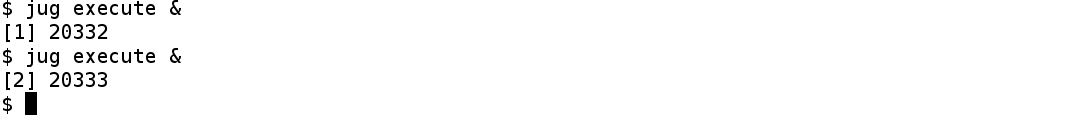
\includegraphics[width=.8\textwidth]{jug_execute}

\end{frame}

\begin{frame}[fragile]
\frametitle{Jug Enhances Reproducibility}

\begin{block}{\alert{Dark Side} of Computational Analysis}
\begin{itemize}
\item ``What was the parameter that generated this result? I think it was ½, right? Had to be.''
\item ``Deleted the intermediate results, reran; now everything is different.''
\item ``We cannot reproduce the table in our own paper.''
\end{itemize}
\end{block}

\begin{block}{Advantages of Jug}


\begin{itemize}
\item With jug, changing parameters \alert{will trigger recomputation of all
downstream results}.
\item \alert{jug invalidate} handles all dependencies
\item Unlike \alert{make}, you can use any Python function
\end{itemize}

\end{block}

\end{frame}

\begin{frame}[fragile]
\frametitle{Finding Out More About Jug\ldots}
\begin{itemize}
\item Talk to me \alert{in person}
\item luis@luispedro.org
\item \url{http://github.com/luispedro/jug}\\the code
\item \url{http://jug.rtfd.org}\\read the fine documentation
\end{itemize}

\end{frame}

\end{document}

